% ============================================================
% CSCE 775 — Paper presentation
% Sygkounas, Loutfi, Persson (GECCO 2026)
% Evolutionary Discovery of RL Algorithms via LLMs
% Compile with XeLaTeX (or tectonic).
% ============================================================

\documentclass[10pt, aspectratio=169]{beamer}
\usetheme{uofsc}
\usepackage{booktabs}
\usepackage{colortbl}
\usepackage{amsmath,amssymb}
\usepackage{tikz}
\usetikzlibrary{shapes.geometric, arrows.meta, positioning, fit, backgrounds, calc, shapes.symbols}
\usepackage{graphicx}
\usepackage{hyperref}

\graphicspath{{figs/}}

% --- Presentation Metadata ---
\title[Evolving RL via LLMs]{Evolutionary Discovery of Reinforcement\\Learning Algorithms via Large Language Models}
\subtitle{Sygkounas, Loutfi \& Persson --- GECCO 2026}
\author[J.C. Vaught]{J.C. Vaught\texorpdfstring{\\}{, }CSCE 775 --- Paper Presentation\texorpdfstring{\\}{, }University of South Carolina}
\institute[UofSC]{}
\date{}

% --- Helpful color shortcuts ---
\newcommand{\hilite}[1]{{\color{UofSCGarnet}\textbf{#1}}}

% ============================================================
\begin{document}

% ------ Title Slide ------
{
  \setbeamertemplate{footline}{}
  \begin{frame}[plain]
    \titlepage
  \end{frame}
}

% ============================================================
% No Introduction divider — jump straight to content.
\section*{Introduction}

% --- S2a: What RL is used for ---
\begin{frame}{What RL is used for}
  \vspace{0.4em}
  \centering
  \begin{tikzpicture}[
    tile/.style={rectangle, draw=UofSCGarnet, line width=1pt, fill=UofSCGray10,
                 minimum width=6.4cm, minimum height=2.3cm, align=center, font=\normalsize,
                 text width=6.1cm}
  ]
    \node[tile] (a) at (0, 0)    {\textbf{Reasoning LLMs}\\[0.2em]
        \scriptsize o1, DeepSeek-R1 --- RL makes them \textit{think}};
    \node[tile] (b) at (7, 0)    {\textbf{LLM alignment}\\[0.2em]
        \scriptsize RLHF, DPO, GRPO, Constitutional AI};
    \node[tile, draw=UofSCGarnet, line width=1.8pt, fill=UofSCSandstorm]
         (c) at (0, -2.8) {\textbf{\color{UofSCGarnet}Robotics \& autonomy}\\[0.2em]
        \scriptsize $\pi_0$, OpenVLA, Atlas, Waymo, AlphaStar};
    \node[tile] (d) at (7, -2.8) {\textbf{Science \& operations}\\[0.2em]
        \scriptsize AlphaDev, AlphaTensor, chip design, data-center cooling};
  \end{tikzpicture}

  \vspace{0.6em}
  \centering
  {\small\color{UofSCGarnet}\textbf{This paper targets \textit{control RL}}
  {\color{UofSCGray70}\normalfont --- Gymnasium / MuJoCo; \textit{not} LLM-RL.}}
\end{frame}

% --- S2b: RL vs ES at a glance ---
\begin{frame}{RL vs.\ ES at a glance}
  \vspace{0.1em}
  \begin{columns}[T]
    \begin{column}{0.48\textwidth}
      \begin{tikzpicture}
        \node[rectangle, draw=UofSCGarnet, line width=1.3pt, fill=UofSCGray10,
              inner sep=0.7em, text width=6.3cm, font=\small] {%
          \textbf{\color{UofSCGarnet}Reinforcement Learning}\\[0.3em]
          {\scriptsize Learn a policy by trial \& error, updated with gradients on a scalar reward.}\\[0.6em]
          \textbf{Where it runs today}\\[0.2em]
          \hspace{0.3em}$\bullet$\; AlphaGo, AlphaStar, MuZero\\
          \hspace{0.3em}$\bullet$\; ChatGPT / Claude / Gemini (RLHF)\\
          \hspace{0.3em}$\bullet$\; o1, DeepSeek-R1 reasoning\\
          \hspace{0.3em}$\bullet$\; Humanoid locomotion, manipulation\\[0.4em]
          {\scriptsize\color{UofSCGray70}\itshape The dominant paradigm.}};
      \end{tikzpicture}
    \end{column}
    \begin{column}{0.48\textwidth}
      \begin{tikzpicture}
        \node[rectangle, draw=UofSCHoneycomb, line width=1.3pt, fill=UofSCGray10,
              inner sep=0.7em, text width=6.3cm, font=\small] {%
          \textbf{\color{UofSCHoneycomb}Evolutionary Search}\\[0.3em]
          {\scriptsize Maintain a population, mutate \& recombine, keep the fittest. No gradients.}\\[0.6em]
          \textbf{Where it runs today}\\[0.2em]
          \hspace{0.3em}$\bullet$\; Neural architecture search (NAS)\\
          \hspace{0.3em}$\bullet$\; Hyperparameter tuning (PBT, PB2)\\
          \hspace{0.3em}$\bullet$\; Reward discovery (Eureka, REvolve)\\
          \hspace{0.3em}$\bullet$\; Non-differentiable problems (FunSearch)\\[0.4em]
          {\scriptsize\color{UofSCGray70}\itshape The niche tool --- used where RL can't go.}};
      \end{tikzpicture}
    \end{column}
  \end{columns}
\end{frame}

% --- S2c: The problem with RL ---
\begin{frame}{The problem with RL}
  \vspace{-0.1em}
  \centering
  \begin{tikzpicture}
    \node[rectangle, draw=UofSCGarnet, line width=1.3pt, fill=UofSCGray10,
          inner sep=0.6em, text width=13cm, font=\small] {%
      \textbf{\color{UofSCGarnet}The same handful of template families keeps getting recycled.}
      LLM alignment has DPO / GRPO / ORPO / SimPO / KTO, but those are all
      preference-weighted PG. For \textbf{control RL} (this paper's domain),
      DQN '15, PPO '17, SAC '18, TD3 '18 are still the workhorses.};
  \end{tikzpicture}

  \vspace{0.5em}
  \begin{columns}[T]
    \begin{column}{0.48\textwidth}
      {\small\textbf{\color{UofSCRose}Sample efficiency}}
      \begin{itemize}\setlength\itemsep{0em}
        \item[\textcolor{UofSCRose}{\tiny$\blacksquare$}] \small PPO / SAC: $\mathbf{10^6\text{--}10^7}$ env steps on MuJoCo
        \item[\textcolor{UofSCRose}{\tiny$\blacksquare$}] \small Humans: $\mathbf{\sim 10^2}$ steps
      \end{itemize}

      \vspace{0.3em}
      {\small\textbf{\color{UofSCRose}Reproducibility}}
      \begin{itemize}\setlength\itemsep{0em}
        \item[\textcolor{UofSCRose}{\tiny$\blacksquare$}] \small $\mathbf{3\times}$ return swings from seeds \& HPs
        \item[\textcolor{UofSCRose}{\tiny$\blacksquare$}] \small PPO impls disagree across codebases
      \end{itemize}
    \end{column}
    \begin{column}{0.48\textwidth}
      {\small\textbf{\color{UofSCRose}Fragility}}
      \begin{itemize}\setlength\itemsep{0em}
        \item[\textcolor{UofSCRose}{\tiny$\blacksquare$}] \small Reward hacking, credit-assignment drift
        \item[\textcolor{UofSCRose}{\tiny$\blacksquare$}] \small Deadly triad: bootstrap + FA + off-policy
      \end{itemize}

      \vspace{0.3em}
      {\small\textbf{\color{UofSCRose}Human bottleneck}}
      \begin{itemize}\setlength\itemsep{0em}
        \item[\textcolor{UofSCRose}{\tiny$\blacksquare$}] \small New algorithm $=$ 1--2 yrs of PhD work
        \item[\textcolor{UofSCRose}{\tiny$\blacksquare$}] \small The update rule has never been automated
      \end{itemize}
    \end{column}
  \end{columns}
\end{frame}

% --- S2d: The problem with ES ---
\begin{frame}{The problem with ES}
  \vspace{-0.1em}
  \centering
  \begin{tikzpicture}
    \node[rectangle, draw=UofSCHoneycomb, line width=1.3pt, fill=UofSCGray10,
          inner sep=0.6em, text width=13cm, font=\small] {%
      \textbf{\color{UofSCHoneycomb}ES is powerful but boxed in by the designer} ---
      flexible and parallel, yet stuck with the search space you wrote down.};
  \end{tikzpicture}

  \vspace{0.5em}
  \begin{columns}[T]
    \begin{column}{0.48\textwidth}
      {\small\textbf{\color{UofSCRose}Sample cost}}
      \begin{itemize}\setlength\itemsep{0em}
        \item[\textcolor{UofSCRose}{\tiny$\blacksquare$}] \small $\mathbf{3\text{--}10\times}$ more env steps than A3C / PPO
        \item[\textcolor{UofSCRose}{\tiny$\blacksquare$}] \small No gradient, no bootstrap, no TD reuse
      \end{itemize}

      \vspace{0.3em}
      {\small\textbf{\color{UofSCRose}Dimensionality}}
      \begin{itemize}\setlength\itemsep{0em}
        \item[\textcolor{UofSCRose}{\tiny$\blacksquare$}] \small Stalls past $\mathbf{\sim 10^6}$ parameters
        \item[\textcolor{UofSCRose}{\tiny$\blacksquare$}] \small RL scales to billions of params
      \end{itemize}
    \end{column}
    \begin{column}{0.48\textwidth}
      {\small\textbf{\color{UofSCRose}Search space}}
      \begin{itemize}\setlength\itemsep{0em}
        \item[\textcolor{UofSCRose}{\tiny$\blacksquare$}] \small DSL / primitives are hand-designed
        \item[\textcolor{UofSCRose}{\tiny$\blacksquare$}] \small Cannot express what you didn't foresee
      \end{itemize}

      \vspace{0.3em}
      {\small\textbf{\color{UofSCRose}Blind mutations}}
      \begin{itemize}\setlength\itemsep{0em}
        \item[\textcolor{UofSCRose}{\tiny$\blacksquare$}] \small Random perturbations waste evals
        \item[\textcolor{UofSCRose}{\tiny$\blacksquare$}] \small No semantic guidance on what to change
      \end{itemize}
    \end{column}
  \end{columns}
\end{frame}

% --- S2e: Demo 1 - RL wins on a clean maze ---
\begin{frame}{Demo --- when RL wins}
  \vspace{0.3em}
  \begin{columns}[T]
    \begin{column}{0.62\textwidth}
      \centering
      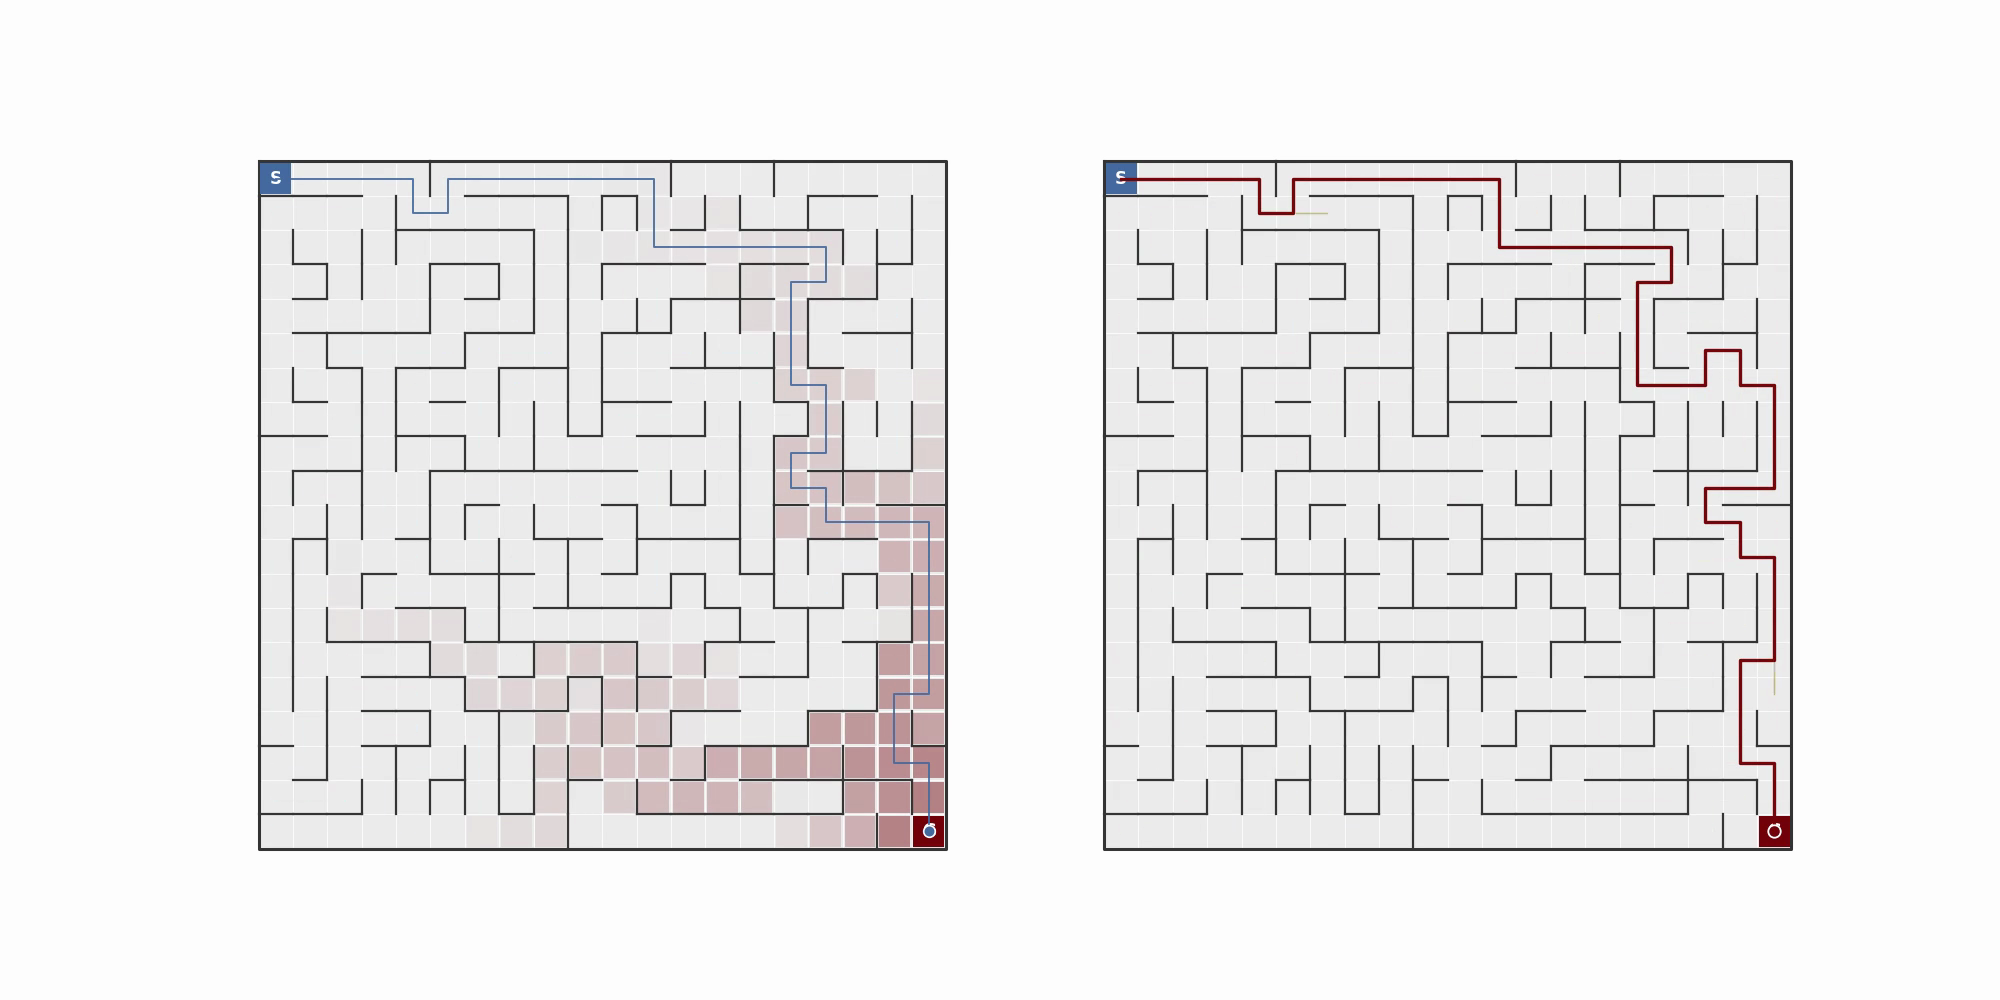
\includegraphics[width=\linewidth]{viz/still_no_traps.png}
    \end{column}
    \begin{column}{0.36\textwidth}
      \vspace{1.3em}
      Same 20$\times$20 maze, sparse goal reward.\\[0.6em]
      \begin{itemize}\setlength\itemsep{0.15em}
        \item RL: 212K env steps, $\sim$50-step path
        \item ES: \hilite{24$\times$ more env steps} for the same result
      \end{itemize}
      \vspace{0.6em}
      {\small\color{UofSCGray70}\itshape Clean credit assignment is RL's home turf.}
    \end{column}
  \end{columns}
\end{frame}

% --- S2f: Demo 2 - ES wins on a deceptive maze ---
\begin{frame}{Demo --- when ES wins}
  \vspace{0.3em}
  \begin{columns}[T]
    \begin{column}{0.62\textwidth}
      \centering
      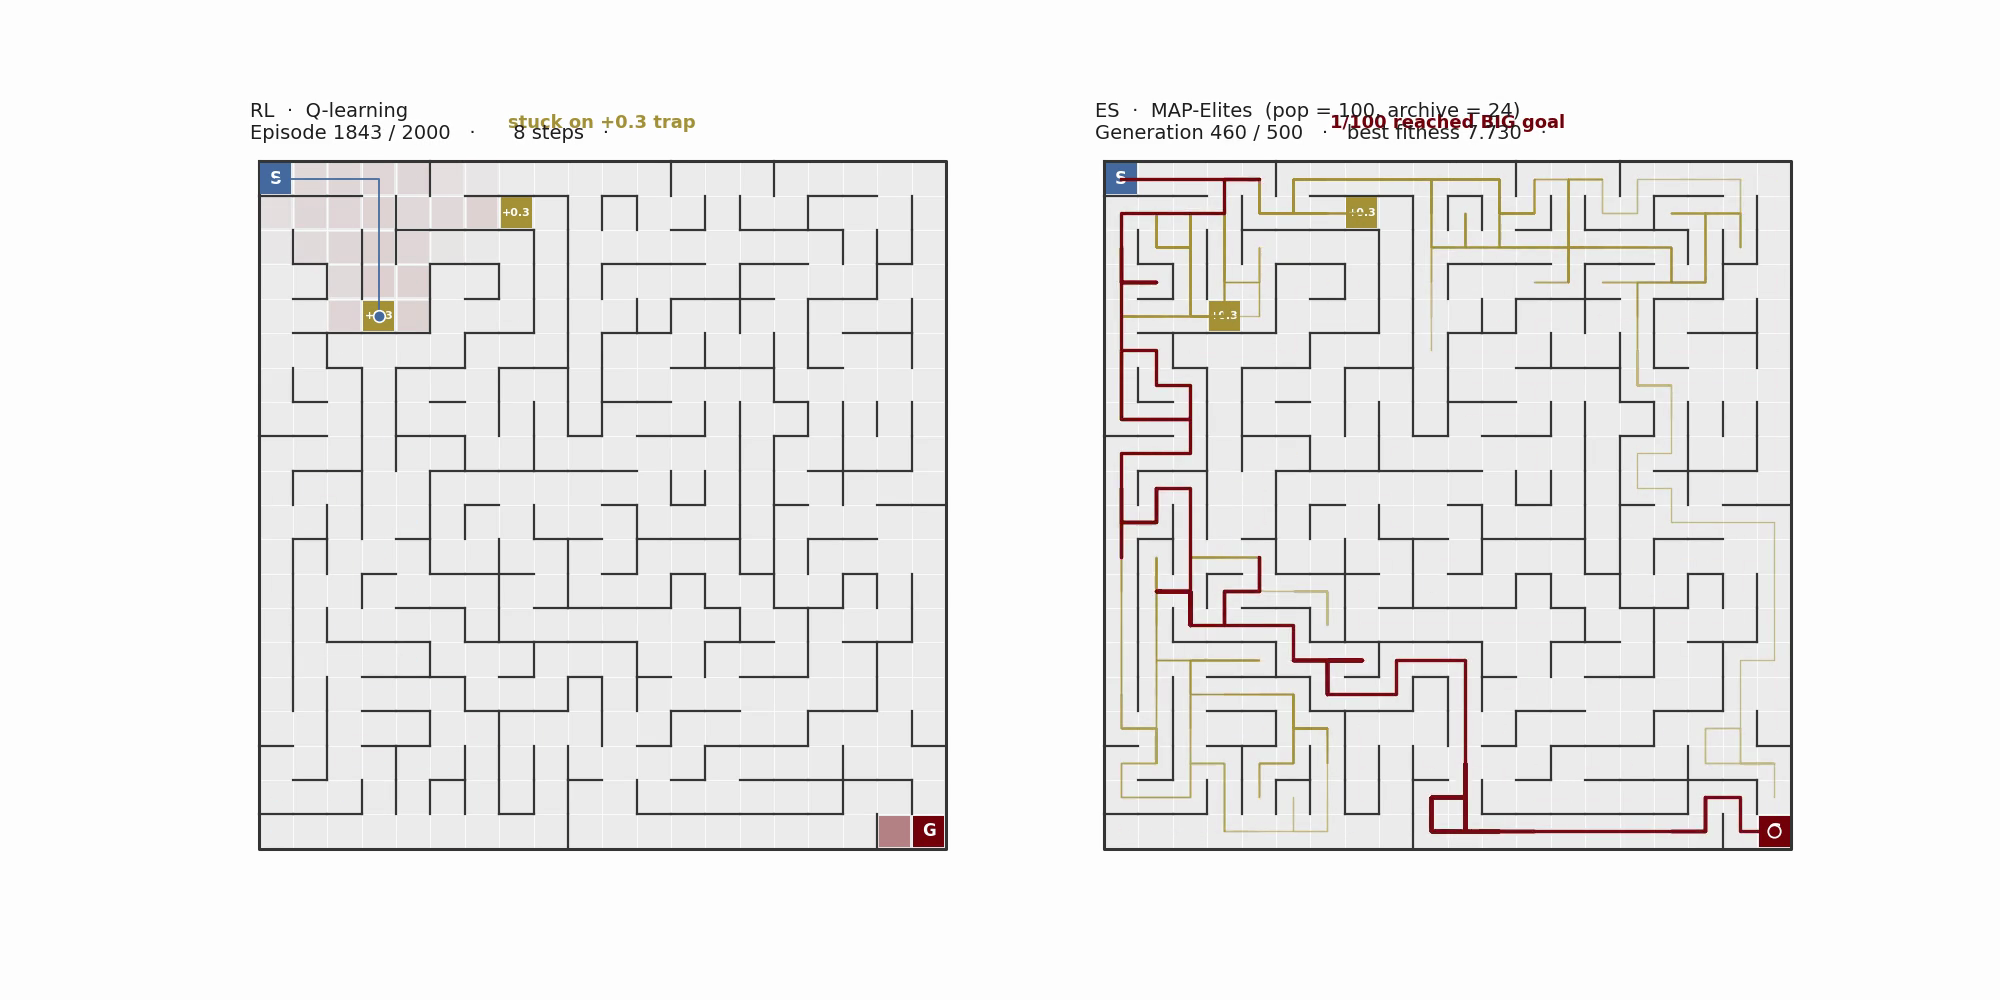
\includegraphics[width=\linewidth]{viz/still_traps.png}
    \end{column}
    \begin{column}{0.36\textwidth}
      \vspace{1.3em}
      Add two small ``trap'' rewards near the start.\\[0.6em]
      \begin{itemize}\setlength\itemsep{0.15em}
        \item RL: \hilite{0\,/\,2{,}000} episodes reach the big goal
        \item ES (MAP-Elites): \hilite{248\,/\,1{,}000} generations do
        \item 302 total breakthroughs $\cdot$ first at gen 44
      \end{itemize}
      \vspace{0.6em}
      {\small\color{UofSCGray70}\itshape Deceptive landscapes are where population search wins.}
    \end{column}
  \end{columns}
\end{frame}

% --- S2: what the paper is ---
\begin{frame}{What this paper is}
  \vspace{0.2em}
  \begin{tikzpicture}
    \node[rectangle, draw=UofSCGarnet, line width=1.4pt, fill=UofSCSandstorm,
          inner sep=0.8em, text width=13.8cm, font=\small] {%
      \textbf{\color{UofSCGarnet}Evolutionary Discovery of Reinforcement Learning
      Algorithms via Large Language Models}\\[0.2em]
      Sygkounas, Loutfi \& Persson --- \"Orebro University --- GECCO 2026};
  \end{tikzpicture}

  \vspace{0.5em}
  \textbf{\color{UofSCGarnet}What they build.}\;
  {\small An evolutionary framework where each candidate is an executable
  Python \texttt{compute\_loss} function defining a complete RL training loop.
  An LLM (GPT-5.2 / Claude 4.5 Opus) proposes mutations and crossovers over
  that code; each variant is scored by actually training agents in Gymnasium.}

  \vspace{0.35em}
  \textbf{\color{UofSCGarnet}How it extends prior work.}\;
  {\small Takes REvolve's LLM-as-variation-operator machinery and points it
  at the \textit{loss function} instead of the \textit{reward function}.
  Prompt-level constraints forbid actor--critic, value functions, and Bellman
  updates so the search has to invent something new.}

  \vspace{0.35em}
  \textbf{\color{UofSCGarnet}What they find.}\;
  {\small Two evolved algorithms --- \textbf{\color{UofSCAtlantic}CG-FPD} and
  \textbf{\color{UofSCCongaree}DF-CWP-CP} --- both planning-style, both
  gradient-free of any classical RL signal. Competitive with PPO and SAC
  across 10 Gymnasium benchmarks after a post-evolution LLM-guided
  hyperparameter pass.}
\end{frame}

% --- S3: why automate RL algorithm design ---
\begin{frame}{Modern RL rests on 5 rules}
  \centering
  \vspace{0.4em}
  \begin{tikzpicture}[
    algbox/.style={rectangle, draw=UofSCGarnet, line width=1pt, fill=UofSCGray10,
                   minimum width=1.8cm, minimum height=1.2cm, font=\bfseries},
    yearlbl/.style={font=\small\color{UofSCGray70}}
  ]
    \node[algbox] (dqn)  at (0,0)   {DQN};
    \node[algbox] (trpo) at (2.1,0) {TRPO};
    \node[algbox] (ddpg) at (4.2,0) {DDPG};
    \node[algbox] (ppo)  at (6.3,0) {PPO};
    \node[algbox] (sac)  at (8.4,0) {SAC};
    \node[algbox] (td3)  at (10.5,0){TD3};

    \node[yearlbl] at (dqn.south)  [below=0.1cm] {2015};
    \node[yearlbl] at (trpo.south) [below=0.1cm] {2015};
    \node[yearlbl] at (ddpg.south) [below=0.1cm] {2015};
    \node[yearlbl] at (ppo.south)  [below=0.1cm] {2017};
    \node[yearlbl] at (sac.south)  [below=0.1cm] {2018};
    \node[yearlbl] at (td3.south)  [below=0.1cm] {2018};
  \end{tikzpicture}

  \vspace{2.4em}
  {\large A decade of progress --- \hilite{hand-designed update rules}.}\\[0.4em]
  {\color{UofSCGray70}\textit{Each took months of PhD-level effort. Each became dogma.}}
\end{frame}

% --- S4: what has been automated — the ladder ---
\begin{frame}{AutoML climbs the ladder}
  \centering
  \vspace{-0.2em}
  \begin{tikzpicture}[
    rung/.style={rectangle, draw=UofSCGray50, line width=0.8pt,
                 minimum width=9cm, minimum height=0.8cm, font=\small,
                 text width=8.4cm},
    crown/.style={rectangle, draw=UofSCGarnet, line width=1.6pt, fill=UofSCGarnet,
                 text=white, minimum width=9cm, minimum height=0.95cm, font=\bfseries,
                 text width=8.4cm}
  ]
    \node[rung] (s1) at (0, 0)    {Architecture \hfill \textit{\color{UofSCGray70}NAS, AmoebaNet}};
    \node[rung] (s2) at (0, 0.95) {Hyperparameters \hfill \textit{\color{UofSCGray70}PB2, OptFormer}};
    \node[rung] (s3) at (0, 1.9)  {Reward function \hfill \textit{\color{UofSCGray70}Eureka, REvolve}};
    \node[rung] (s4) at (0, 2.85) {Preference loss \hfill \textit{\color{UofSCGray70}DiscoPOP}};
    \node[crown](s5) at (0, 3.9)  {The update rule itself \hfill ???};
    \draw[-{Stealth[length=3mm]}, UofSCGarnet, line width=1.4pt]
      ($(s4.north)+(0,0.03)$) -- ($(s5.south)-(0,0.03)$);
  \end{tikzpicture}

  \vspace{0.6em}
  {\large The \hilite{loss function} was the last frontier.}
\end{frame}

% ============================================================
\sectionsubtitle{Two lineages converge on one idea}
\section{Background}

% --- S5: Lineage A ---
\begin{frame}{Lineage A: Discover an RL algorithm}
  \centering
  \vspace{0.2em}
  \begin{tikzpicture}[
    node distance=0.4cm,
    chev/.style={signal, signal to=east, signal pointer angle=135, draw=UofSCAtlantic,
                 fill=UofSCAtlantic, text=white, line width=0.8pt, minimum width=2.4cm,
                 minimum height=1.0cm, font=\bfseries\small},
    tagbox/.style={font=\footnotesize\itshape\color{UofSCGray70}, align=center, text width=2.6cm}
  ]
    \node[chev] (a) at (0,0)  {EPG '18};
    \node[chev] (b) at (3.2,0){LPG '20};
    \node[chev] (c) at (6.4,0){Co-Reyes '21};
    \node[chev] (d) at (9.6,0){DiscoRL '25};

    \node[tagbox, below=0.15cm of a] {neural loss for PG};
    \node[tagbox, below=0.15cm of b] {LSTM update rule};
    \node[tagbox, below=0.15cm of c] {DAG over typed ops};
    \node[tagbox, below=0.15cm of d] {meta-learned NN (Nature)};
  \end{tikzpicture}

  \vspace{2.5em}
  \begin{center}
    \begin{tikzpicture}
      \node[rectangle, draw=UofSCGarnet, line width=1.2pt, fill=UofSCGray10,
            inner sep=0.8em, font=\large] {%
        All \hilite{constrain the search space by hand}.};
    \end{tikzpicture}
  \end{center}
\end{frame}

% --- S6: Lineage B ---
\begin{frame}{Lineage B: LLMs mutate code}
  \centering
  \vspace{0.2em}
  \begin{tikzpicture}[
    chev/.style={signal, signal to=east, signal pointer angle=135, draw=UofSCHoneycomb,
                 fill=UofSCHoneycomb, text=white, line width=0.8pt, minimum width=2.6cm,
                 minimum height=1.0cm, font=\bfseries\small},
    tagbox/.style={font=\footnotesize\itshape\color{UofSCGray70}, align=center, text width=2.8cm}
  ]
    \node[chev] (a) at (0,0)   {ELM '22};
    \node[chev] (b) at (3.4,0) {FunSearch '24};
    \node[chev] (c) at (6.8,0) {AlphaEvolve '25};
    \node[chev] (d) at (10.2,0){EvoTune '25};

    \node[tagbox, below=0.15cm of a] {LLMs as mutators};
    \node[tagbox, below=0.15cm of b] {cap-set, bin-packing};
    \node[tagbox, below=0.15cm of c] {full files, Strassen beaten};
    \node[tagbox, below=0.15cm of d] {proposer fine-tuning};
  \end{tikzpicture}

  \vspace{2.2em}
  \begin{center}
    \begin{tikzpicture}
      \node[rectangle, draw=UofSCGarnet, line width=1.2pt, fill=UofSCGray10,
            inner sep=0.8em, font=\large] {%
        LLMs are \hilite{intelligent variation operators} over code.};
    \end{tikzpicture}
  \end{center}
\end{frame}

% --- S7: REvolve ---
\begin{frame}{Parent work: REvolve (2024)}
  \begin{columns}[T]
    \begin{column}{0.55\textwidth}
      \vspace{0.6em}
      \begin{tikzpicture}[
        node distance=0.5cm,
        bx/.style={rectangle, draw=UofSCGarnet, line width=1pt, fill=UofSCGray10,
                   minimum width=3.2cm, minimum height=0.85cm, font=\small},
        llm/.style={rectangle, draw=UofSCCongaree, line width=1pt, fill=UofSCCongaree,
                    text=white, minimum width=3.2cm, minimum height=0.85cm, font=\small\bfseries},
        arr/.style={-{Stealth[length=3mm]}, UofSCGarnet, line width=1pt}
      ]
        \node[bx]  (pop)  {Population of $R(s,a)$};
        \node[llm] (mut)  [below=of pop] {GPT-4 mutate / crossover};
        \node[bx]  (train) [below=of mut] {Train RL agent};
        \node[bx]  (eval)  [below=of train] {Human preference (Elo)};

        \draw[arr] (pop)   -- (mut);
        \draw[arr] (mut)   -- (train);
        \draw[arr] (train) -- (eval);
        \draw[arr] (eval.east) -- ++(1.0,0) |- (pop.east);
      \end{tikzpicture}
    \end{column}
    \begin{column}{0.43\textwidth}
      \vspace{1.2em}
      \textbf{What REvolve evolves}
      \begin{itemize}
        \item Executable Python \hilite{reward functions}
        \item Island populations, LLM variation
        \item Tested on driving, humanoid, dexterous hands
      \end{itemize}
      \vspace{0.8em}
      \begin{tikzpicture}
        \node[rectangle, draw=UofSCGarnet, line width=1.2pt, fill=UofSCSandstorm,
              inner sep=0.6em, text width=5.2cm, font=\small] {%
          \textbf{The move in this paper.}\\
          Evolve the \hilite{loss function} instead of the reward.};
      \end{tikzpicture}
    \end{column}
  \end{columns}
\end{frame}

% --- S8: thesis slide ---
\begin{frame}{The gap this paper fills}
  \centering
  \vspace{0.2em}
  \begin{tabular}{@{}l c l@{}}
    \toprule
    \textbf{What gets evolved} & & \textbf{Representative method} \\
    \midrule
    Architecture            & \checkmark & NAS, AmoebaNet \\
    Hyperparameters         & \checkmark & PB2, OptFormer \\
    Reward function         & \checkmark & REvolve, Eureka \\
    Preference loss (align) & \checkmark & DiscoPOP \\
    Update rule (DAG)       & \checkmark & Co-Reyes 2021 \\
    Update rule (black-box NN) & \checkmark & LPG, DiscoRL \\
    \midrule
    \rowcolor{UofSCSandstorm}
    \textbf{\color{UofSCGarnet}Update rule (executable Python, LLM-evolved)}
                            & \textbf{\color{UofSCGarnet}$\bigstar$}
                            & \textbf{\color{UofSCGarnet}Sygkounas et al. 2026} \\
    \bottomrule
  \end{tabular}

  \vspace{1.2em}
  {\large Everything above is \textit{context}. The bottom row is \hilite{the thesis}.}
\end{frame}

% ============================================================
\sectionsubtitle{How the framework works}
\section{Method}

% --- S9: hero method figure ---
\begin{frame}{The big picture}
  \begin{columns}[T]
    \begin{column}{0.58\textwidth}
      \vspace{0.5em}
      \centering
      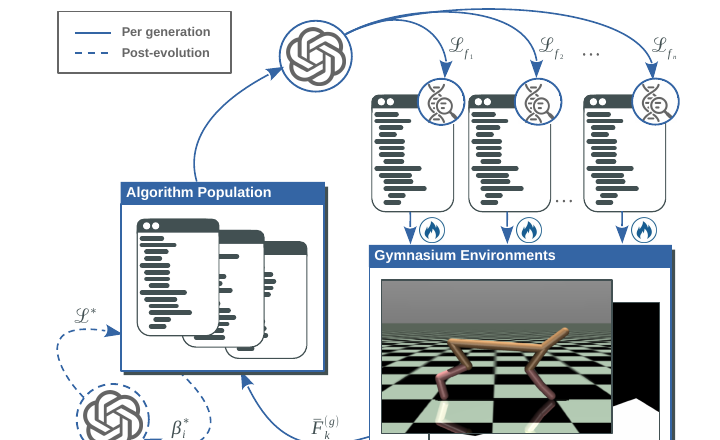
\includegraphics[width=\linewidth]{fig1_method.png}
    \end{column}
    \begin{column}{0.40\textwidth}
      \vspace{1.4em}
      \textbf{Per generation}
      \begin{itemize}
        \item LLM proposes candidate loss functions
        \item Each is trained end-to-end on 5 Gym envs
        \item Fitness drives selection
      \end{itemize}

      \vspace{0.8em}
      \textbf{Post-evolution}
      \begin{itemize}
        \item LLM proposes hyperparameter ranges
        \item Sweep finds the refined rule $\mathcal{L}^{\star}$
      \end{itemize}
    \end{column}
  \end{columns}
  \vfill
  {\footnotesize\color{UofSCGray70}\textit{Figure 1 from the paper.}}
\end{frame}

% --- S10: what a candidate looks like ---
\begin{frame}{A candidate is a chunk of Python}
  \begin{columns}[T]
    \begin{column}{0.48\textwidth}
      \centering\textbf{Parent}\\[0.4em]
      \begin{tikzpicture}
        \node[rectangle, draw=UofSCGray50, line width=0.8pt, fill=UofSCGray10,
              inner sep=0.8em, text width=6.1cm, font=\ttfamily\scriptsize] {%
          def compute\_loss(theta, xi, D):\\
          \hspace{1em}preds = model(D.s, theta)\\
          \hspace{1em}targets = rollout(model, D.s)\\
          \hspace{1em}L = mse(preds, targets)\\
          \hspace{1em}return L};
      \end{tikzpicture}
    \end{column}
    \begin{column}{0.48\textwidth}
      \centering\textbf{After LLM mutation}\\[0.4em]
      \begin{tikzpicture}
        \node[rectangle, draw=UofSCGarnet, line width=1pt, fill=UofSCSandstorm,
              inner sep=0.8em, text width=6.1cm, font=\ttfamily\scriptsize] {%
          def compute\_loss(theta, xi, D):\\
          \hspace{1em}preds = model(D.s, theta)\\
          \hspace{1em}\textbf{\color{UofSCGarnet}conf = xi.confidence(D.s)}\\
          \hspace{1em}targets = rollout(model, D.s)\\
          \hspace{1em}\textbf{\color{UofSCGarnet}L = (conf * mse(preds, targets)).mean()}\\
          \hspace{1em}return L};
      \end{tikzpicture}
    \end{column}
  \end{columns}

  \vspace{1.2em}
  \centering
  {\large The LLM \hilite{edits Python}. That is the entire search space.}
\end{frame}

% --- S11: evolutionary loop ---
\begin{frame}{The evolutionary loop}
  \centering
  \begin{tikzpicture}[
    stepbox/.style={rectangle, draw=UofSCGarnet, line width=1.2pt, fill=UofSCGray10,
                 minimum width=3.2cm, minimum height=1.6cm, align=center, font=\small},
    arr/.style={-{Stealth[length=3.5mm]}, UofSCGarnet, line width=1.2pt}
  ]
    \node[stepbox] (s1) at (0,2.2)   {\textbf{1. Select parents}\\{\scriptsize from island pool}};
    \node[stepbox] (s2) at (6.2,2.2) {\textbf{2. LLM varies code}\\{\scriptsize mutate $p{=}0.65$}\\{\scriptsize crossover $p{=}0.35$}};
    \node[stepbox] (s3) at (6.2,-0.8){\textbf{3. Train on 5 envs}\\{\scriptsize 3 seeds each}};
    \node[stepbox] (s4) at (0,-0.8)  {\textbf{4. Rank by fitness}\\{\scriptsize replace weakest}};

    \draw[arr] (s1) -- (s2);
    \draw[arr] (s2) -- (s3);
    \draw[arr] (s3) -- (s4);
    \draw[arr] (s4) -- (s1);

    \node[rectangle, draw=UofSCCongaree, line width=1pt, fill=white,
          minimum width=2.4cm, minimum height=1.2cm, align=center, font=\small\itshape]
      at (3.1,0.7) {diversity-aware\\Levenshtein\\crossover};
  \end{tikzpicture}

  \vspace{0.6em}
  {\color{UofSCGray70}\small Island model $\cdot$ 9 individuals per island $\cdot$ 24 new candidates per generation.}
\end{frame}

% --- S12: forbidden mechanisms ---
\begin{frame}{What the LLM is told not to do}
  \centering
  \vspace{0.3em}
  \begin{tikzpicture}[
    forbid/.style={rectangle, draw=UofSCRose, line width=1.6pt, fill=UofSCGray10,
                   minimum width=3.6cm, minimum height=2.6cm, align=center, font=\bfseries}
  ]
    \node[forbid] (a) at (0,0)    {No actor--critic\\decomposition};
    \node[forbid] (b) at (4.6,0)  {No bootstrapped\\value targets};
    \node[forbid] (c) at (9.2,0)  {No temporal-\\difference updates};

    \foreach \n in {a,b,c} {
      \node[circle, draw=UofSCRose, line width=1.4pt,
            minimum size=0.9cm] at ($(\n.north west)+(0.55,-0.55)$) (s\n) {};
      \draw[UofSCRose, line width=1.4pt]
        ($(s\n.north west)+(0.12,-0.12)$) -- ($(s\n.south east)+(-0.12,0.12)$);
    }
  \end{tikzpicture}

  \vspace{1.4em}
  {\large Constitutional prompt constraints $\Rightarrow$ \hilite{forces novel mechanisms}.}\\[0.4em]
  {\color{UofSCGray70}\itshape Evolution cannot re-invent DQN; it has to find something else.}
\end{frame}

% --- S13: LLM-HPO ---
\begin{frame}{LLM-guided HPO pass}
  \centering
  \vspace{0.4em}
  \begin{tikzpicture}[
    box/.style={rectangle, draw=UofSCGarnet, line width=1pt, fill=UofSCGray10,
                minimum width=5.8cm, minimum height=3.2cm, font=\small},
    arr/.style={-{Stealth[length=3mm]}, UofSCGarnet, line width=1.2pt}
  ]
    \node[box] (a) at (0,0) {};
    \node[font=\small\bfseries, text=UofSCGarnet] at (0,1.3) {Before LLM-HPO};
    \node[font=\scriptsize\itshape, align=center, text width=5.2cm] at (0,0.1)
         {Evolved rule works\\ but fitness is noisy across\\ hyperparameter choices.};

    \node[box, fill=UofSCSandstorm] (b) at (8,0) {};
    \node[font=\small\bfseries, text=UofSCGarnet] at (8,1.3) {After LLM-HPO};
    \node[font=\scriptsize\itshape, align=center, text width=5.2cm] at (8,0.1)
         {LLM proposes bounded\\ interval $[\ell_j, u_j]$ per scalar.\\ Sweep $\Rightarrow$ refined rule $\mathcal{L}^{\star}$.};

    \draw[arr] (a) -- (b);
  \end{tikzpicture}

  \vspace{0.8em}
  {\color{UofSCGray70}\small Policy arch, optimizer, rollout loop stay frozen. Only internal scalars move.}
\end{frame}

% ============================================================
\sectionsubtitle{What evolution discovered}
\section{Results}

% --- S14: two algorithms ---
\begin{frame}{The two algorithms it invented}
  \centering
  \vspace{0.2em}
  \begin{columns}[T]
    \begin{column}{0.47\textwidth}
      \begin{tikzpicture}
        \node[rectangle, draw=UofSCAtlantic, line width=1.4pt, fill=UofSCGray10,
              inner sep=0.9em, text width=6.3cm, font=\small] {%
          \textbf{\color{UofSCAtlantic}CG-FPD}\\[0.3em]
          \textbf{Confidence-Guided Forward Policy Distillation}\\[0.6em]
          Distill short-horizon plans from a learned latent dynamics model.
          Planning acts as the supervised teacher signal.\\[0.4em]
          \textit{\color{UofSCGray70}No value function. No policy gradient. No Bellman.}};
      \end{tikzpicture}
    \end{column}
    \begin{column}{0.47\textwidth}
      \begin{tikzpicture}
        \node[rectangle, draw=UofSCCongaree, line width=1.4pt, fill=UofSCGray10,
              inner sep=0.9em, text width=6.3cm, font=\small] {%
          \textbf{\color{UofSCCongaree}DF-CWP-CP}\\[0.3em]
          \textbf{Differentiable Forward Confidence-Weighted Planning with Controllability Prior}\\[0.6em]
          Differentiable world-model rollouts + confidence-weighted desirability + controllability prior.\\[0.4em]
          \textit{\color{UofSCGray70}Also avoids every canonical RL mechanism.}};
      \end{tikzpicture}
    \end{column}
  \end{columns}

  \vspace{1.2em}
  {\large Evolution rediscovered \hilite{model-based planning} --- from scratch.}
\end{frame}

% --- S15: fitness curves ---
\begin{frame}{The proposer LLM matters. A lot.}
  \begin{columns}[T]
    \begin{column}{0.58\textwidth}
      \vspace{0.2em}
      \centering
      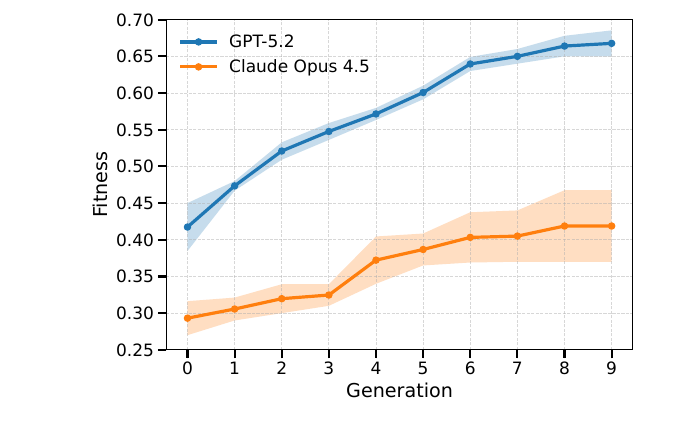
\includegraphics[width=\linewidth]{fig3_fitness.png}
    \end{column}
    \begin{column}{0.40\textwidth}
      \vspace{1.6em}
      \begin{itemize}
        \item GPT-5.2 climbs to \hilite{0.67}
        \item Claude 4.5 Opus caps at \hilite{0.42}
        \item Both monotone; GPT-5.2 is sharper on every generation
      \end{itemize}

      \vspace{1em}
      {\color{UofSCGray70}\itshape Same framework, same envs, same seeds --- just swap the LLM.}
    \end{column}
  \end{columns}
\end{frame}

% --- S16: benchmark table ---
\begin{frame}{Results match PPO and SAC}
  \centering
  \vspace{0.2em}
  \begin{tabular}{@{}lcccc@{}}
    \toprule
    \textbf{Environment} & \textbf{PPO} & \textbf{SAC} & \textbf{\color{UofSCAtlantic}CG-FPD} & \textbf{\color{UofSCCongaree}DF-CWP-CP} \\
    \midrule
    CartPole          & 500.0  & ---      & \textbf{500.0}  & \textbf{500.0} \\
    LunarLander       & 246.6  & ---      & 241.2           & \textbf{260.6} \\
    MountainCar       & $-128.1$ & ---    & \textbf{$-105.8$} & \textbf{$-108.6$} \\
    Acrobot           & $-63.5$ & ---     & \textbf{$-90.6$} & $-78.6$ \\
    HalfCheetah       & 1579.1 & 4988.5  & 2407.9          & 2103.8 \\
    Swimmer           & 95.0   & 87.8    & 247.5           & 219.8 \\
    Walker2d          & 3163.2 & 4595.3  & 1603.8          & 1297.6 \\
    InvertedPendulum  & 1000.0 & 1000.0  & \textbf{1000.0} & \textbf{1000.0} \\
    \bottomrule
  \end{tabular}

  \vspace{0.8em}
  {\large Competitive with hand-designed baselines \hilite{across 10 environments}.}\\[0.3em]
  {\color{UofSCGray70}\small Evolved on 5 training envs; remaining 5 are generalization tests.}
\end{frame}

% --- S17: alpha ablation ---
\begin{frame}{Ablation: diversity weight}
  \begin{columns}[T]
    \begin{column}{0.58\textwidth}
      \centering
      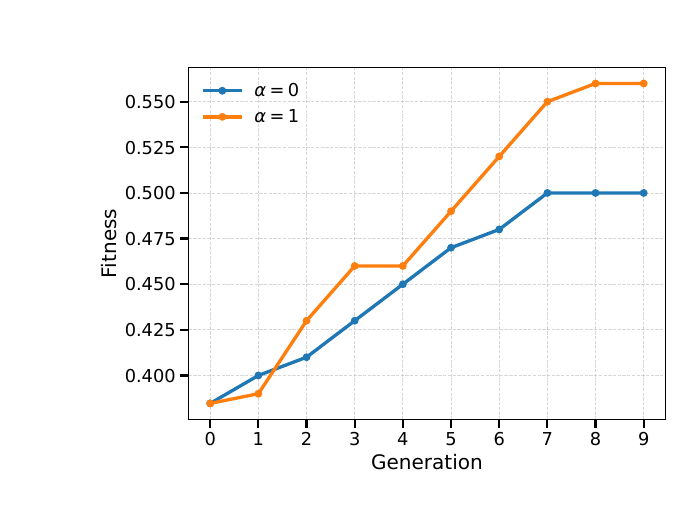
\includegraphics[width=0.96\linewidth]{fig5_alpha.png}
    \end{column}
    \begin{column}{0.40\textwidth}
      \vspace{1.2em}
      \textbf{Levenshtein weight $\alpha$}
      \begin{itemize}
        \item $\alpha = 0$: no structural regularization $\Rightarrow 0.50$
        \item $\alpha = 1$: full regularization $\Rightarrow 0.56$
        \item $\alpha = 0.5$: \hilite{$0.65$}
      \end{itemize}

      \vspace{0.8em}
      {\color{UofSCGray70}\itshape Some code-similarity nudge helps; too much or too little hurts.}
    \end{column}
  \end{columns}
\end{frame}

% ============================================================
\sectionsubtitle{Critique and open questions}
\section{Discussion}

% --- S18: strengths / weaknesses ---
\begin{frame}{Strengths vs. weaknesses}
  \begin{columns}[T]
    \begin{column}{0.48\textwidth}
      \textbf{\color{UofSCGarnet}Strengths}
      \vspace{0.3em}
      \begin{itemize}
        \item First \hilite{full update-rule} discovery via LLM
        \item Genuinely novel mechanisms (no value, no PG)
        \item Clean extension of REvolve's machinery
        \item LLM-HPO handles fitness fragility cleanly
      \end{itemize}
    \end{column}
    \begin{column}{0.48\textwidth}
      \textbf{\color{UofSCRose}Weaknesses}
      \vspace{0.3em}
      \begin{itemize}
        \item 30\,h per candidate on 4$\times$A100
        \item Narrow benchmarks (CartPole / MuJoCo only)
        \item Is GPT-5.2 \textit{discovering} or \textit{remembering}?
        \item Only 2 evolutionary seeds per LLM
        \item No head-to-head vs.\ DiscoRL
        \item Constitutional constraints never ablated
      \end{itemize}
    \end{column}
  \end{columns}
\end{frame}

% --- S19: 2x2 matrix ---
\begin{frame}{Where this paper sits in the field}
  \centering
  \vspace{0.2em}
  \begin{tikzpicture}[
    cell/.style={rectangle, draw=UofSCGarnet, line width=1pt,
                 minimum width=4.6cm, minimum height=2.4cm, align=center, font=\small},
    hl/.style  ={rectangle, draw=UofSCGarnet, line width=1.8pt, fill=UofSCSandstorm,
                 minimum width=4.6cm, minimum height=2.4cm, align=center, font=\small\bfseries},
    axis/.style={font=\small\bfseries, text=UofSCGarnet}
  ]
    \node[axis] at ( 2.3,3.0) {RL};
    \node[axis] at ( 6.9,3.0) {Alignment};
    \node[axis, rotate=90] at (-0.2, 1.6) {NN-parameterized};
    \node[axis, rotate=90] at (-0.2,-0.8) {Code};

    \node[cell] (nnRL)    at ( 2.3, 1.6) {\textbf{DiscoRL}\\ (Oh 2025)\\ meta-learned NN};
    \node[cell] (nnALIGN) at ( 6.9, 1.6) {\textbf{RLHF / DPO}\\ (Rafailov 2023)\\ neural reward model};
    \node[hl]   (codeRL)  at ( 2.3,-0.8) {\color{UofSCGarnet}This paper\\ (Sygkounas 2026)\\ evolved Python};
    \node[cell] (codeAL)  at ( 6.9,-0.8) {\textbf{DiscoPOP}\\ (Lu 2024)\\ LLM-evolved loss};
  \end{tikzpicture}

  \vspace{0.6em}
  {\large The real contest --- \hilite{evolved source code} vs.\ \hilite{meta-gradient} for RL.}
\end{frame}

% --- S20: future directions ---
\begin{frame}{Open questions}
  \vspace{0.4em}
  \begin{itemize}
    \item \textbf{Surrogate fitness} to break the 30\,h/candidate wall.
    \item \textbf{Lift the constraints} --- let evolution \textit{decide} whether to re-use actor--critic.
    \item \textbf{Scale to Atari and robotics} --- generalization is still untested.
    \item \textbf{Curriculum over environments} --- connect to POET, XLand.
    \item \textbf{Self-improving proposer} --- EvoTune-style DPO on the evolved database.
  \end{itemize}

  \vspace{1.6em}
  \begin{center}
    \begin{tikzpicture}
      \node[rectangle, draw=UofSCGarnet, line width=1.4pt, fill=UofSCSandstorm,
            inner sep=0.9em, text width=12cm, align=center, font=\itshape] {%
        \textbf{Takeaway.} REvolve showed LLMs can evolve rewards.
        This paper shows they can evolve the \textbf{entire algorithm}.
        The open question is whether what they discover is genuinely new ---
        or just a good remix of what the model already saw.};
    \end{tikzpicture}
  \end{center}
\end{frame}

% ============================================================
% Thank You / Q&A
% ============================================================
{
  \setbeamertemplate{footline}{}
  \begin{frame}[plain]
    \begin{tikzpicture}[remember picture, overlay]
      \fill[UofSCGarnet] (current page.south west) rectangle (current page.north east);
      \fill[UofSCDarkGarnet] (current page.south west) rectangle ([yshift=0.8cm]current page.south east);
      \draw[white, line width=0.5pt] ([yshift=0.8cm]current page.south west) -- ([yshift=0.8cm]current page.south east);
    \end{tikzpicture}
    \vfill
    \centering
    {\fontsize{50}{55}\selectfont\impactfont\color{UofSCWhite} THANK YOU!}\\[1em]
    {\Large\color{UofSCWhite} Questions \& Discussion}\\[0.5em]
    {\normalsize\color{UofSCGray30} jvaught@sc.edu}
    \vfill
  \end{frame}
}

\end{document}
